\documentclass[UTF8]{ctexart}
\usepackage{graphicx}
\usepackage{amsmath}
\usepackage{float}
\pagestyle{plain}   
% \usepackage{booktabs}
% \usepackage{subfigure}
\usepackage{setspace}
\date{}
\title{机器学习lab1} 
\author{杨景凯}
\date{2022/10/27} 
\begin{document} 
% \maketitle 
\begin{center}
    \quad \\
    \quad \\
    \kaishu \fontsize{45}{17} 上\quad 海\quad 交\quad 通\quad 大\quad 学
    \vskip 3.5cm
    \heiti \zihao{2} 机器学习\\
    lab1
\end{center}
\vskip 3.5cm
\begin{quotation}
    \songti \fontsize{30}{30}
    \doublespacing
    \par\setlength\parindent{12em}
    \quad 
\begin{center}
    % 学\hspace{0.61cm} 院:\underline{电子信息与电气工程学院}

    学生姓名:\underline{\qquad    \quad \quad 杨景凯    \quad  \quad\qquad }

    学\hspace{0.61cm} 号:\underline{\quad \quad\quad520021910550\quad\quad}

\end{center}
    
    \centering
    2022年10月27日
\end{quotation}
\clearpage
\tableofcontents
\clearpage
\section{基本介绍}
\subsection{目的}
本次Lab主要是实现两种方法的SVM模型并对比其准确度和时间。其中,两种方法分别是:使用sklearn包中的线性SVM模型和使用梯度下降法的手动实现的SVM模型。
\subsection{环境}
\subsubsection{python环境}
本次使用的python版本为3.7.9 64bit。
\subsubsection{包环境}
通过pip freeze将环境生成requirements.txt文件,如下所示:
\begin{itemize}
    \item $numpy==1.21.4$
    \item $scikit\_learn==1.1.3$
\end{itemize}
\subsubsection{机器环境}
理论上,本代码在所有64bit的机器上均能正常运行。本次实验所用的环境为:
\begin{itemize}
    \item CPU: Intel(R) Core(TM) i5-6300U CPU @ 2.40GHz   2.50 GHz
    \item RAM: 4GB 1867MHZ
\end{itemize}
\section{SVM-sklearn}
\subsection{实现方法}
通过初始化SVM线性模型,并输入训练数据,其能自动训练。将测试数据输入模型,得到准确度。准确度的计算方式是,模型计算出的预测值与实际值差的绝对值的平均。
\subsection{参数}
经过测试与选取,我选择了如下参数:
\begin{itemize}
    \item $THRESHOLD = 1^{-3}$
    \item $MAX\_ITERATION = -1$
\end{itemize}
其中,选择$THRESHOLD = 1^{-3}$是为了在保证时间较短情况下增加准确度,选择$MAX\_ITERATION = -1$是为了避免其提早结束导致准确度骤降(若选择和梯度下降相同的最大迭代次数,即8000次,则其准确度只有0.71,并抛出警告其提前结束)
\subsection{结果}
根据上述参数配置,得到结果如下:
\begin{itemize}
    \item $train\_acc: 0.975$
    \item $test\_acc: 0.91$
    \item $Running\ time: 1.3125 Second$
\end{itemize}
同时可以画出准确度与时间随$THRESHOLD$的变化图如下:
\begin{figure}[H]
    \centering
    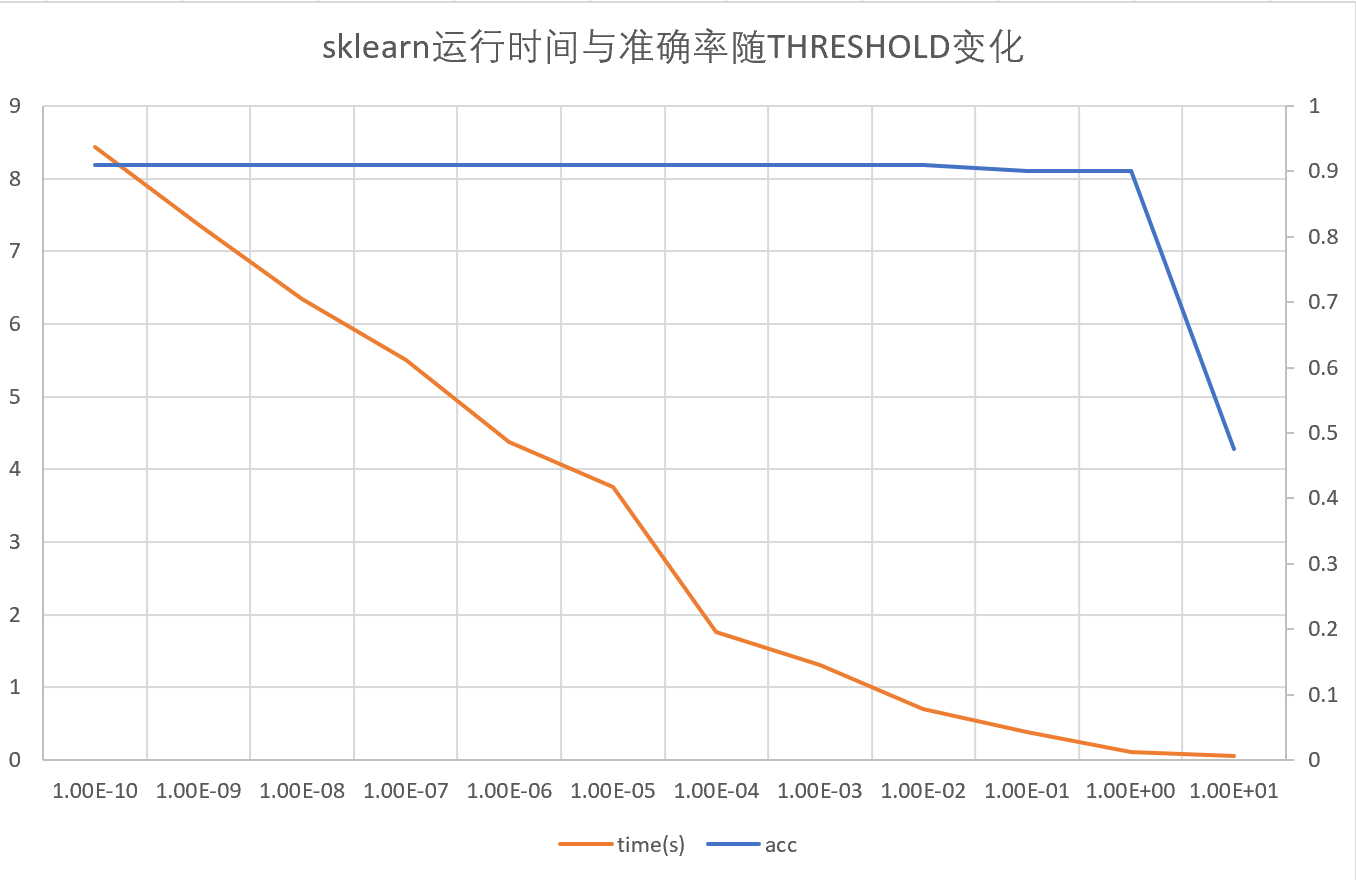
\includegraphics[scale=0.6]{./img/sklearn.png}
    \caption{sklearn准确度与时间随THRESHOLD变化图}
\end{figure}
可以发现,其在THRESHOLD约为$1 \cdot 10^{-3}$时达到稳定,此时运行时间为1.3125s,准确率为0.91。
最终结果为:
\begin{align}
    w=[&-2.802051483528587,0.06326673,0.07667397,0.18258601,0.60309771,\nonumber\\
    &-0.28708404,-0.20567921,0.4027636,-0.65930869,-0.84561177,\nonumber\\
    &-0.81467686,0.52399726,-0.67723609,-0.20361242 -0.44343857,\nonumber\\
    &-0.22124865,0.50415385,-0.41556441,-0.12376121,0.01310567,\nonumber\\
    &-0.51855263,-0.5626143,0.44617828,0.50301771,-0.07107305,\nonumber\\
    &-0.2538178,0.99309579,0.52277441,0.00215304,0.00112656]\nonumber
\end{align}

\section{SVM-gradient decent}
\subsection{实现方法}
几乎相同于课堂上展示的伪代码,但是使用np与矩阵来进行计算,加速计算速度也减少代码量。
最终的损失函数为:
$$L(w,w_0|D)=\left\{
    \begin{aligned}
&\frac{\lambda}{2} ||w||^2 &y^{(l)}(w^Tx^{(l)}+w_0)\geq 1\\
&\frac{1}{N}\Sigma_{l=1}^N 1-y^{(l)}(w^Tx^{(l)}+w_0)+\frac{\lambda}{2} ||w||^2 & otherwise\\
\end{aligned}
\right.$$
其中,$\lambda$表示为下述PENALTY。
详细地,方法为:
\begin{enumerate}
    \item 随机产生初始的w值。
    \item 对于$w_1-w_N$,首先计算所有满足$y^{(l)}(w^Tx^{(l)}+w_0)\geq 1$对应的下标集合$I$,对于每个下标,计算$\Delta w_j=-\frac{1}{N} \cdot \Sigma_{i \in I}x_j^{(i)}\cdot y^{(i)}+PENALTY \cdot w_j$。对于$w_0$,$\Delta w_0 = -\Sigma_{i \in I}y^{(i)}$。
    \item 更新$w_0=w_0-STEP\_SIZE \cdot \Delta w_0$,$w=w-STEP\_SIZE \cdot \Delta w$。
\end{enumerate}
将测试数据输入模型,得到准确度。准确度的计算方式是,模型计算出的预测值与实际值差的绝对值的平均。同时由于初始随机性的选取,我将代码运行5次,准确度与时间计算取平均值。
\subsection{参数}
经过测试与选取,我选择了如下参数:
\begin{itemize}
    \item $PENALTY = 0.001$
    \item $THRESHOLD = 1^{-9}$
    \item $STEP\_SIZE = 0.0003$
    \item $MAX\_ITERATION = 8000$
\end{itemize}
其中,选择$PENALTY = 0.001$是为了降低w的平方和的占比,选择$THRESHOLD = 1^{-9}$和$MAX\_ITERATION = 8000$是为了在保证时间较短情况下增加准确度,选择$STEP\_SIZE = 0.0003$是为了增加准确度,使得其缓慢迭代。
\subsection{结果}
根据上述参数配置,得到结果如下:
\begin{itemize}
    \item $train\_acc: 0.9325$
    \item $test\_acc: 0.92$
    \item $Running\ time: 2.78125 Second$
\end{itemize}
同时可以画出当$MAX\_ITERATION = 8000$时准确度与时间随THRESHOLD的变化图如下:
\begin{figure}[H]
    \centering
    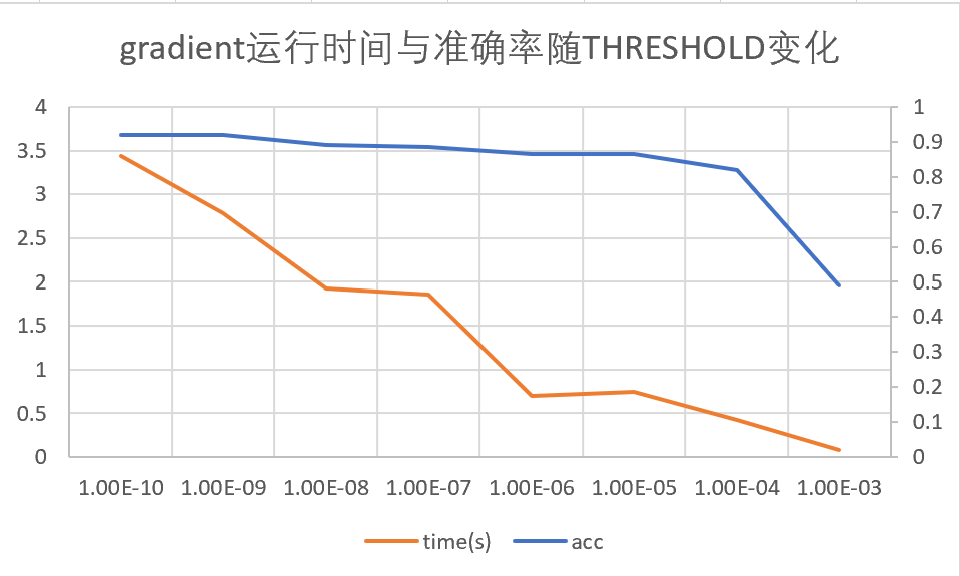
\includegraphics[scale=0.8]{./img/gradient.png}
    \caption{gradient准确度与时间随THRESHOLD变化图}
\end{figure}
可以发现,其在$THRESHOLD$约为$1 \cdot 10^{-9}$时达到稳定。同时,设置为此值时,迭代次数差不多为8000(当设置为$1 \cdot 10^{-8}$时,迭代次数约为4000)。
同时,也可以画出准确度与时间随$STEP\_SIZE$变化图如下:
\begin{figure}[H]
    \centering
    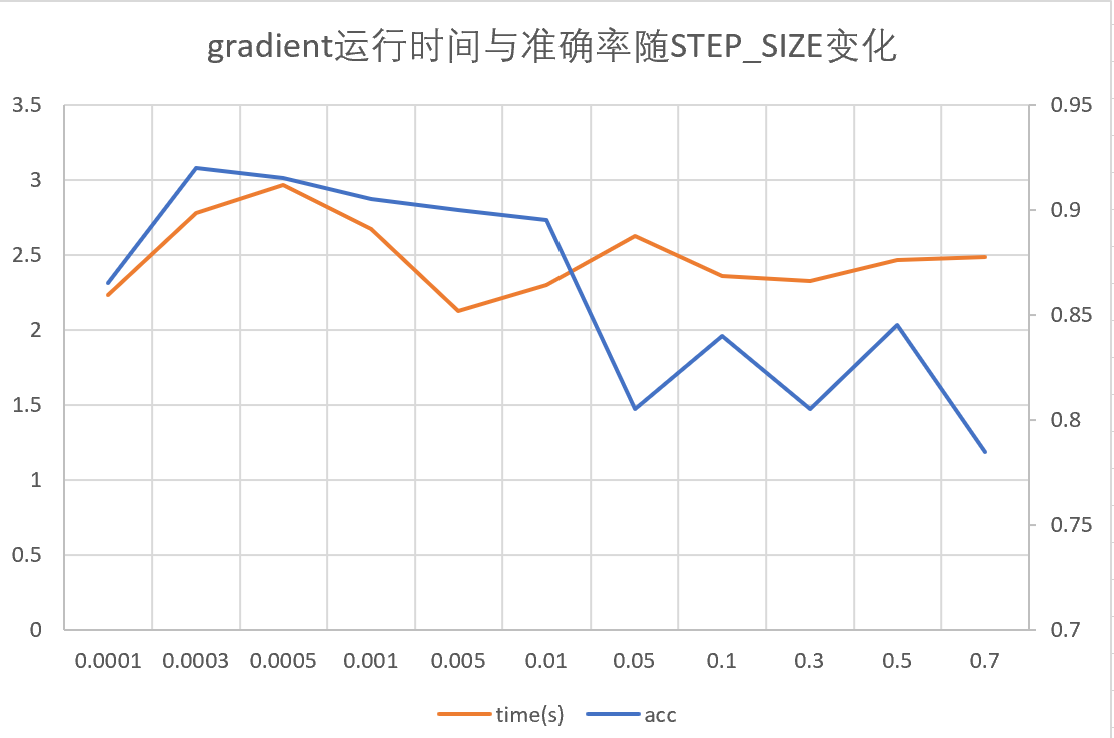
\includegraphics[scale=0.8]{./img/gradient_step_size.png}
    \caption{gradient准确度与时间随$STEP\_SIZE$变化图}
\end{figure}
可以发现,其基本保持不变,因此我选择最大值,即$STEP\_SIZE$ = 0.0003。
画出准确度与时间随$PENALTY$变化图如下:
\begin{figure}[H]
    \centering
    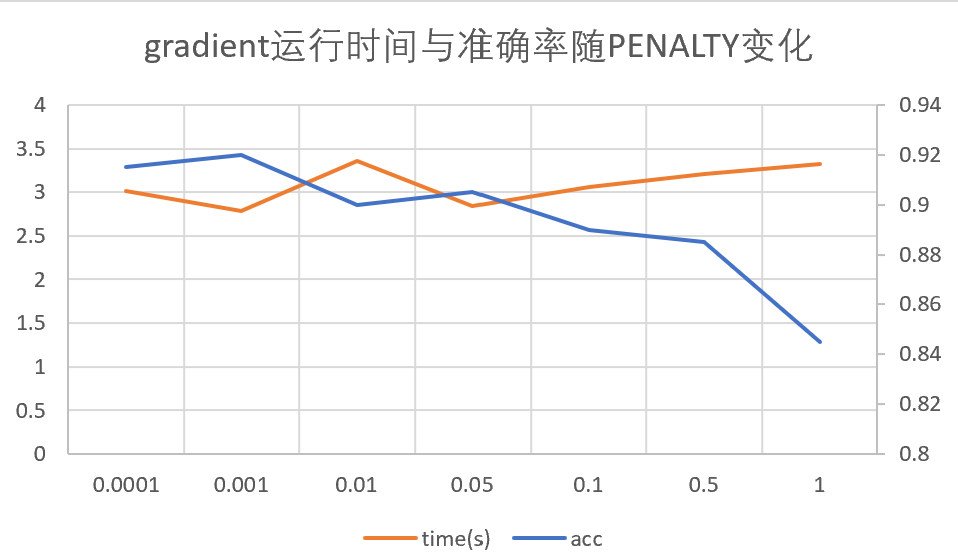
\includegraphics[scale=0.8]{./img/gradient_penalty.png}
    \caption{gradient准确度与时间随PENALTY变化图}
\end{figure}
对于PENALTY来说,由于并未规定取多少,因此我取了可以使得运行时间最短同时准确率最高的0.001。
此时,运行时间为2.78125s,准确率为0.92。
最终结果为:
\begin{align}
    w=[&-0.61092617,-2.29493064e-01,-1.32799101e-02,-2.37979400e-01,2.50455259e-01,\nonumber\\
    &-1.45104633e-01,9.34174521e-02,3.64139625e-02,-1.06806357e-01,-1.27525606e-01,\nonumber\\
    &-1.87934020e-01,1.07382368e-01,-2.22253625e-01,-8.32127053e-02,-2.72055261e-01,\nonumber\\
    &7.61677805e-02,-2.29022182e-02,-1.11535143e-01,3.70389924e-02,-6.91222326e-03,\nonumber\\
    &7.80859202e-03,3.87350089e-02,-2.39034455e-04,-4.33990394e-03,4.08749327e-02,\nonumber\\
    &-3.02514495e-02,1.03504090e-02,3.15397126e-02,-4.06747076e-03,-7.86600723e-04]\nonumber
\end{align}
\subsection{变化}
最终变化情况如图所示:
\begin{figure}[H]
    \centering
    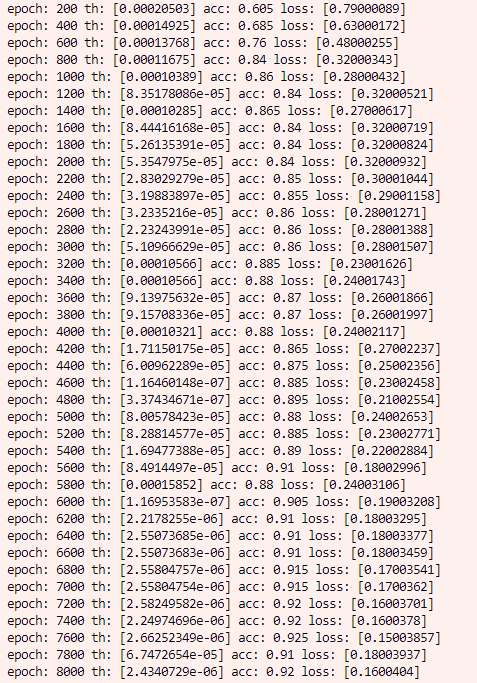
\includegraphics[scale=0.6]{./img/epoch.png}
    \caption{变化情况}
\end{figure}
画图如下所示:
\begin{figure}[H]
    \centering
    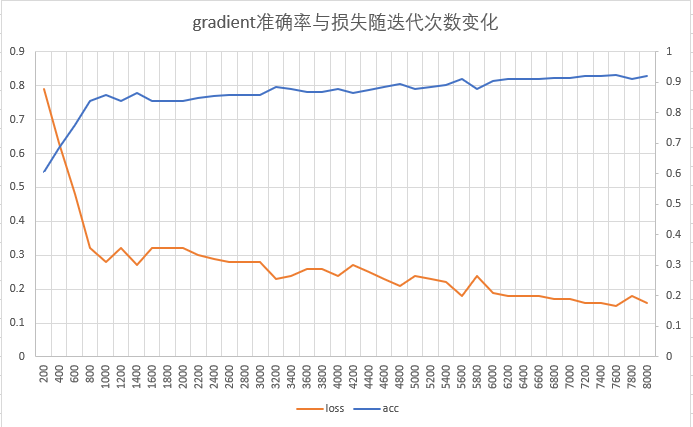
\includegraphics[scale=0.7]{./img/gradient_epoch.png}
    \caption{变化情况}
\end{figure}

\section{对比与分析}
\subsection{时间对比}
从时间上来看,达到相同的准确率需要的时间是sklearn小于使用gradient decent的SVM。我认为有两个原因:
\begin{enumerate}
    \item 加速算法的使用。在计算中可以发现,sklearn的迭代次数远远多于8000次,而仍然能够达到快速,是由于用到了很多加速算法。例如多线程并行计算等。
    \item 底层的不同。在sklearn中,很多函数的编写是使用C来编写的,相比python,C能提供极大的速度加成。
\end{enumerate}
\subsection{准确度对比}
从准确度上看,两者大体相似。在足够迭代后,均能达到90\%以上的准确度,且再增加迭代次数不会发生明显变化。这说明参数已经收敛,几乎达到了最佳的准确度。
\subsection{数据对比}
观察发现,两者最终得出的w不太一致。这是由于不同方法导致的。支持向量选取的不同也会导致这样的结果。
\subsection{结论}
总之,手动编写的使用gradient decent方法的SVM也能达到与sklearn的SVM相似的效果,因此表现了代码的有效性。

% \clearpage
% \begin{thebibliography}{99}  
% \end{thebibliography}
\end{document}
